% Copyright 2020 Glen Newton
% License: Creative Commons Attribution-ShareAlike 4.0 International License https://creativecommons.org/licenses/by-sa/4.0/legalcode
%\documentclass[a0paper,10pt]{article}
\documentclass[12pt]{article}


\usepackage{tikz}
\usepackage[margin=6mm]{geometry}

\usepackage[extreme]{savetrees}
\usepackage{microtype}
\usepackage[hidelinks]{hyperref}
\usetikzlibrary{positioning,shapes,backgrounds}

%\usepackage{atbegshi}% http://ctan.org/pkg/atbegshi
%\AtBeginDocument{\AtBeginShipoutNext{\AtBeginShipoutDiscard}}


% from: https://tex.stackexchange.com/questions/250150/formatting-mindmap-in-tikz
\hypersetup{
  colorlinks=false
}

\definecolor{myb}{rgb}{0, 0, 0.6}

\renewcommand{\familydefault}{\sfdefault}

\newcommand{\boundellipse}[3]% center, xdim, ydim
           {(#1) ellipse (#2 and #3)
           }

% from: https://tex.stackexchange.com/questions/107057/adjusting-font-size-with-tikz-picture

\hypersetup{
  pdftitle={},
  pdfsubject={},
  pdfauthor={Glen Newton},
  pdfkeywords={}
}

\begin{document}

\sffamily
\pagestyle{empty}

{\centering
  \noindent
  \makebox[0pt]{%
    \resizebox{\columnwidth}{!}
              {
                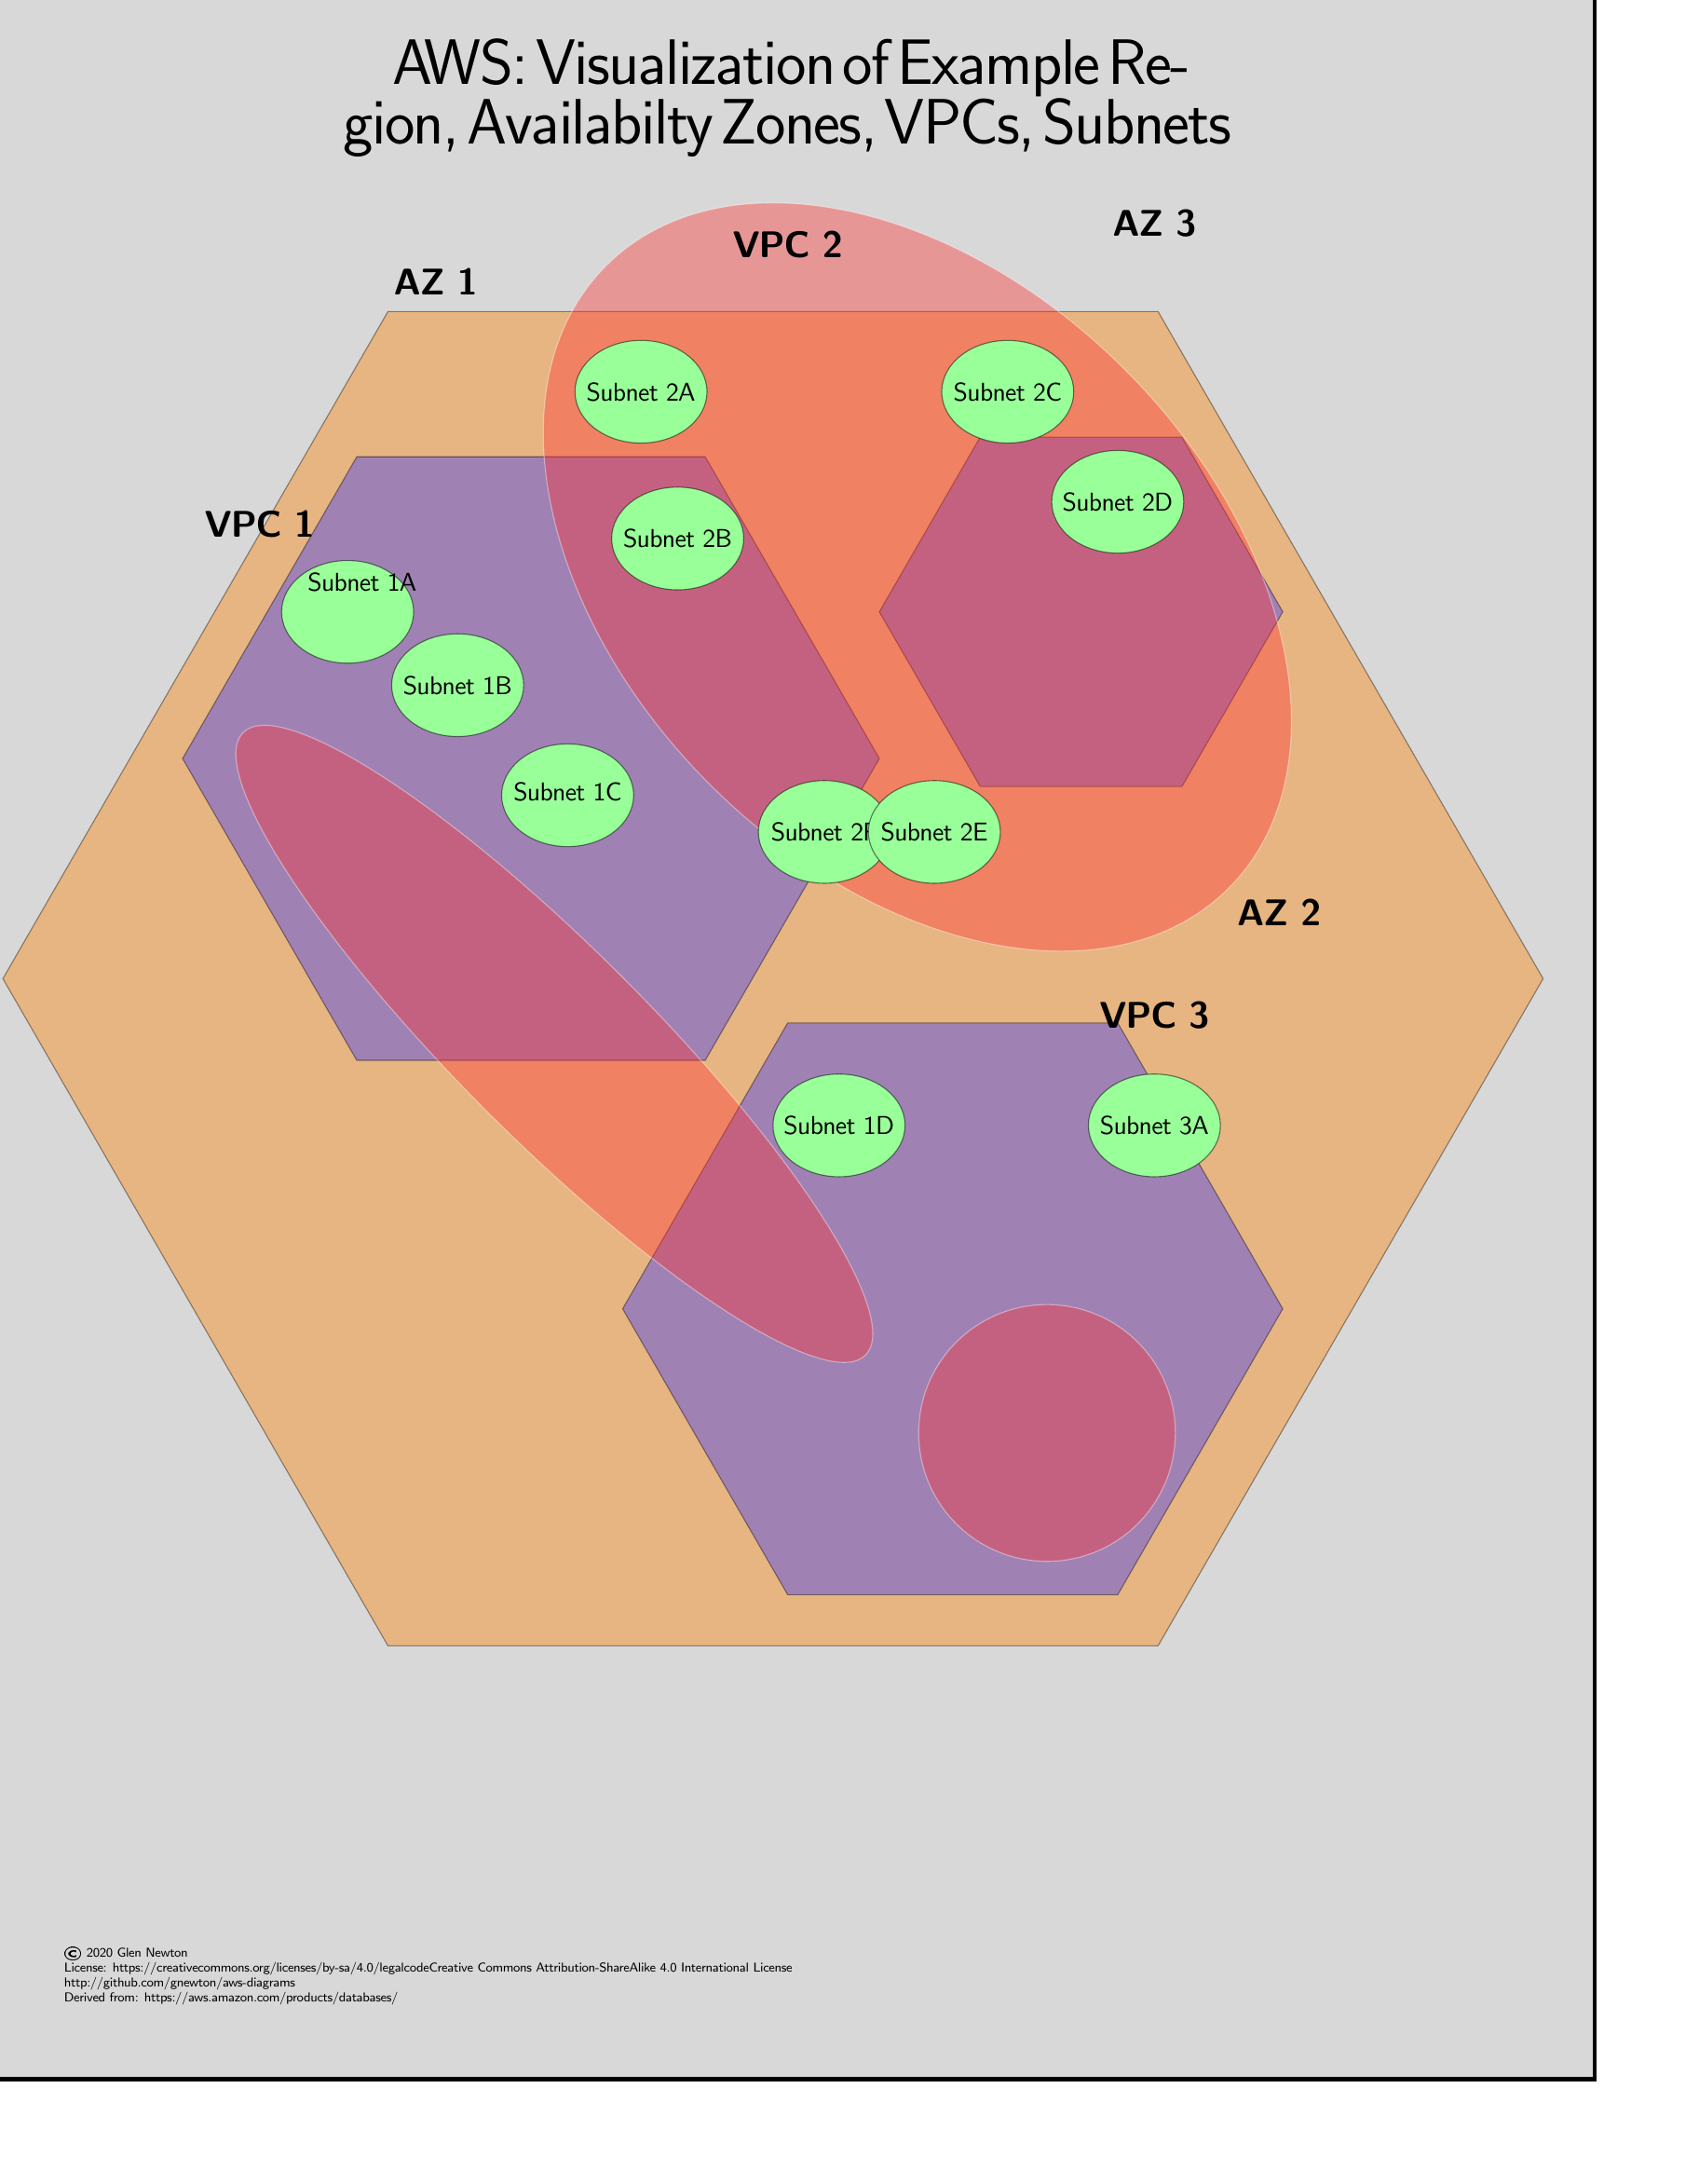
\begin{tikzpicture}
                  \begin{scope}
                    \draw [ultra thick, fill=gray!60, fill opacity=0.5] (-11.4,-18) -- (11,-18) -- (11,11) -- (-11.4,11) -- (-11.4,-18);
                  \end{scope}
                  \begin{scope}[
                      region/.style={color=orange,opacity=0.4,draw=black},
                      az/.style={color=blue!80,opacity=0.4,draw=black},
                      vpc/.style={color=red!80,opacity=0.4,draw=white},
                      subnet/.style={color=green!40,draw opacity=0.5, draw=black},
                      %yshift=-2cm
                    ]
                    \draw (-.2, -3) node[region,regular polygon, regular polygon sides=6, minimum width=21cm, fill ] {};

                    % AZ1
                    \draw (-3.5, 0) node[az,regular polygon, regular polygon sides=6, minimum width=9.5cm, fill ] {};
                    % AZ2
                    \draw (2.25, -7.5) node[az,regular polygon, regular polygon sides=6, minimum width=9cm, fill ] {};
                    % AZ3
                    \draw (4,2) node[az,regular polygon, regular polygon sides=6, minimum width=5.5cm, fill ] {};
                    
                    % VPC1
                    \fill[vpc, rotate=-45] \boundellipse{.5,-5}{6}{1.3};
                    %VPC2
                    \fill[vpc,rotate=45] \boundellipse{3,0.5}{4}{6};
                    %VPC3
                    \fill[vpc,rotate=45] \boundellipse{-4,-9}{1.75}{1.75};

                    \fill[subnet] \boundellipse{-1.5,3}{.9}{.7};
                    \fill[subnet] \boundellipse{-2,5}{.9}{.7};
                    \fill[subnet] \boundellipse{-3,-0.5}{.9}{.7};

                    % 1A
                    \fill[subnet] \boundellipse{-6,2}{.9}{.7};
                    \node at (-5.8,2.4)    {\textsf{Subnet 1A}};

                    % 1B
                    \fill[subnet] \boundellipse{-4.5,1}{.9}{.7};
                    \node at (-4.5,1)    {\textsf{Subnet 1B}};

                    % 1D
                    \fill[subnet] \boundellipse{.7,-5}{.9}{.7};
                    \node at (.7,-5)    {\textsf{Subnet 1D}};

                    % 2F
                    \fill[subnet] \boundellipse{.5,-1}{.9}{.7};
                    \node at (.5,-1)    {\textsf{Subnet 2F}};

                    % 2E
                    \fill[subnet] \boundellipse{2,-1}{.9}{.7};
                    \node at (2,-1)    {\textsf{Subnet 2E}};

                    % 2D
                    \fill[subnet] \boundellipse{4.5,3.5}{.9}{.7};
                    \node at (4.5,3.5)    {\textsf{Subnet 2D}};

                    % 2C
                    \fill[subnet] \boundellipse{3,5}{.9}{.7};
                    \node at (3,5)    {\textsf{Subnet 2C}};

                    
                    \fill[subnet] \boundellipse{5,-5}{.9}{.7};
                    
                    %\node at (0,9.3)    {\textsf{\huge \bf AWS Region}};

                    \node at (-4.8,6.5)    {\textsf{\Large \bf AZ 1}};


                    \node at (-3,-0.45)    {\textsf{Subnet 1C}};



                    \node at (6.7,-2.1)    {\textsf{\Large \bf AZ 2}};
                    \node at (-7.2,3.2)    {\textsf{\Large \bf VPC 1}};
                    \node at (0,7)    {\textsf{\Large \bf VPC 2}};

                    \node at (5,7.3)    {\textsf{\Large\bf AZ 3}};

                    \node at (5,-3.5)    {\textsf{\Large \bf VPC 3}};
                    \node at (5,-5)    {\textsf{Subnet 3A}};

                    \node at (-2,5)    {\textsf{Subnet 2A}};
                    \node at (-1.5,3)    {\textsf{Subnet 2B}};

                    






                    
                  \end{scope}
                  \node[xshift=0cm,yshift=9cm,text width=14cm, align=center](title) {
                    \Huge AWS: Visualization of Example Region, Availabilty Zones, VPCs, Subnets
                  };
                  \node[xshift=-4.9cm,yshift=-16.5cm](foox) {
                    %                  Copyright 2020 Glen Newton
                                      \tiny
                  \begin{tabular}{l}
                  \\
                    \copyright \ 2020 Glen Newton\\
                    License: \href{https://creativecommons.org/licenses/by-sa/4.0/legalcode}{Creative Commons Attribution-ShareAlike 4.0 International License}\\
                    \url{http://github.com/gnewton/aws-diagrams} \\
                    Derived from: \url{https://aws.amazon.com/products/databases/}
                  \end{tabular}

                  };
  \end{tikzpicture}}}\par}


\end{document}
